The \xmlNode{Components} node contains the technical and economic definitions of the components (or
units) within the grid system that needs to be solved. The \xmlNode{Components} node contains many
\xmlNode{Component} nodes defining each of the grid components.

\subsection{Component Activity}
At each time point in a dispatch optimization, HERON attempts to calculate the most optimal usage of
each component in the system. To report the usage of each resource in each unit in the system, HERON
uses some conventions that we explain here.

We can consider two quantities when reporting the activity of a component over time: the quantity of
product consumed or produced, or the rate at which a product is consumed or produced. For instance,
if a Component produces ``widgets'', at a particular hour we can either talk about the total number
of widgets produced during an hour period, or about the rate (in widgets per second) at which they
were produced. Generally, we only track the rate of production for all Components when performing
dispatch optimization; however, for a \xmlNode{Component} who \xmlNode{stores} a resource, we track
the \emph{level} (or \emph{net quantity produced}) instead of the \emph{rate}.

\subsubsection{General Activity}
For most components, when the activity is reported at a particular time for a component, it
represents the instantaneous production level of that component at that time. For example, if a
component's max capacity is given as 10 widgets per second, and the activity reported for hour 2 is
3, then instantaneously at the beginning of hour 2 the unit is assumed to be producing 3 widgets per
second. Simlarly, if a power plant has a capacity of 100 MW and activity is reported as 5 for a
particular hour, then at beginning of that hour the plant is producing 5 MW. Between time points, it
is assumed that the rate of production varies linearly between the reported time points.

\subsubsection{Storage Activity}
Unlike other components, for a storage (a \xmlNode{Component} who \xmlNode{stores} a resource) we
report the instantaneous \emph{level} of the storage instead of the instantaneous production rate.
We formally define the level (or ``net quantity produced'') at a specific time as
\begin{equation}
  L(t) = L_0 + \int_{t_0}^t R(t) dt,
\end{equation}
where:
\begin{itemize}
  \item $L$ is the net quantity produced at time $t$,
  \item $L_0$ is an initial level at the start of the analysis period,
  \item $t$ is the continuous variable for \emph{time},
  \item $t_0$ is the starting time, at which the components has level $L_0$, and
  \item $R(t)$ is the rate of production for the component at time $t$.
\end{itemize}
In discrete terms,
\begin{equation}
  L_k = L_0 + \sum_{i=1}^{k-1} R_i \Delta_k,
\end{equation}
where:
\begin{itemize}
  \item $k$ is an index for discrete time intervals $t_k$,
  \item $L_k$ is the level at the beginning of time interval $t_k$,
  \item $R_k$ is the production rate for the component during time interval $t_k$, and
  \item $\Delta_k$ is the length of the time interval $t_k$.
\end{itemize}
The equivalent continuous production rate for a storage component is therefore
\begin{equation}
  R(t) = \frac{\partial}{\partial t} L(t),
\end{equation}
or, in discrete form given the constant production assumption,
\begin{equation}
  R_k = \frac{L_{k+1} - L_k}{\Delta_k}.
\end{equation}
We want to emphasize this key difference: the \emph{production rate} is interpreted differently for
storage and other producers. For \textbf{storages},
\begin{itemize}
  \item production rate during a time step is considered \emph{discontinuously constant}, and
  \item activity is reported as the \emph{level} of the storage at the beginning of the time step.
\end{itemize}
For \textbf{all other components},
\begin{itemize}
  \item production rate during a time step is considered \emph{continuously linear}, and
  \item activity is reported as the \emph{instantaneous production rate} of the storage at the
        beginning of the time step.
\end{itemize}
This difference has significant impact when developing a \xmlNode{Validator} or plotting dispatch
results. As a demonstration, see Figures \ref{fig:producer_example} and \ref{fig:storage_example}.

In Figure \ref{fig:producer_example}, the black dots indicate the statepoints that HERON reports,
while the green dashed line is the assumed production between statepoints. Note the
$y$-axis is in units of production rate.

\begin{figure}[h!]
  \centering
  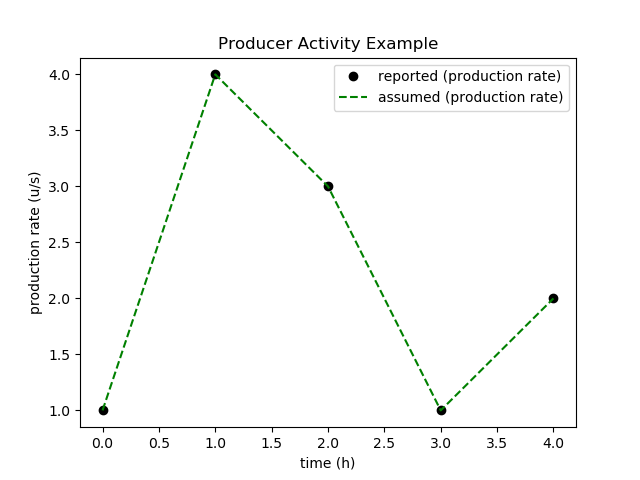
\includegraphics[width=0.5\textwidth]{../pics/producer_activity_explained.png}
  \caption{Producer Example}
  \label{fig:producer_example}
\end{figure}

In Figure \ref{fig:storage_example}, the black dots indicate the statepoints that HERON reports,
with units of emph{level}, not production rate. The red dotted line is the assumed level between
statepoints, and the green dashed lines are the equivalent production between each statepoint.
Note the dual $y$-axis: one is in units of production rate (green, left), while the other is in units of level or
quantity (red, right). That is, the storage unit filly slowly, then fills quickly, then totally depletes before
filling again. This same activity can be represented by the production rates in the dashed green
lines, with negative production indicating absorbing into storage and positive production indicating
emission from storage.
\begin{figure}[h!]
  \centering
  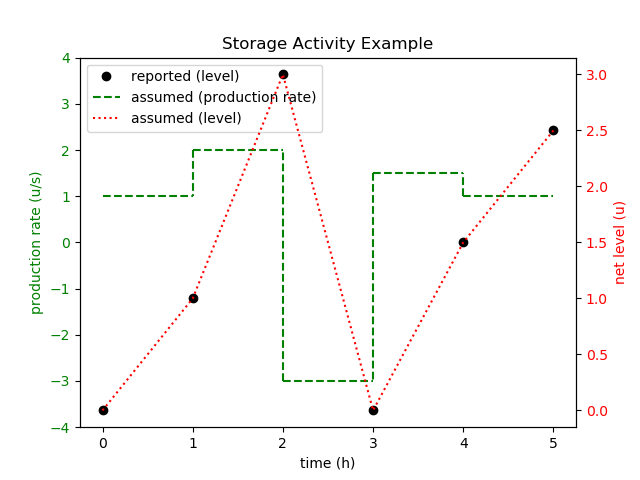
\includegraphics[width=0.5\textwidth]{../pics/storage_activity_explained.png}
  \caption{Storage Example}
  \label{fig:storage_example}
\end{figure}
